\documentclass[conference]{IEEEtran}

% Note: 
% The layout of this tex file was generated by GenAI (chatgpt), based on a picture of the template provided for this paper.

% ------------------------------------------------------------
% PAGE LAYOUT
% ------------------------------------------------------------
\usepackage[paperwidth=210mm,paperheight=297mm,
            left=20mm, right=15mm, top=25mm, bottom=20mm,
            columnsep=5mm]{geometry}

% ------------------------------------------------------------
% FONTS & ENCODING
% ------------------------------------------------------------
\usepackage[T1]{fontenc}
\usepackage[utf8]{inputenc}
\usepackage{times}                % Times New Roman-like text
\usepackage{microtype}            % better justification

% ------------------------------------------------------------
% SECTION TITLES
% ------------------------------------------------------------
\usepackage{titlesec}
% Sections in SMALL CAPS, 12pt, centered
\titleformat*{\section}{\normalfont\scshape\centering\small}
\titleformat*{\subsection}{\normalfont\bfseries\small}

% ------------------------------------------------------------
% ABSTRACT & KEYWORDS
% ------------------------------------------------------------
\usepackage{abstract}
\renewcommand{\abstractnamefont}{\normalfont\bfseries\small}  % "Abstract"
\renewcommand{\abstracttextfont}{\normalfont\itshape\small}   % body
\setlength{\absleftindent}{0pt}
\setlength{\absrightindent}{0pt}

\newcommand{\keywords}[1]{%
  \vspace{1ex}\par\noindent%
  \textbf{Keywords—}\small #1%
}

% ------------------------------------------------------------
% CAPTIONS
% ------------------------------------------------------------
\usepackage[font=small,labelfont=bf,labelsep=period,justification=centering]{caption}

% ------------------------------------------------------------
% TEXT
% ------------------------------------------------------------
\usepackage[utf8]{inputenc}
\usepackage{enumitem}

% ------------------------------------------------------------
% GRAPHICS
% ------------------------------------------------------------
\usepackage{float}
\usepackage{graphicx}

% ------------------------------------------------------------
% HYPERREF (optional)
% ------------------------------------------------------------
\usepackage[hidelinks]{hyperref}

% ------------------------------------------------------------
% TITLE BLOCK
% ------------------------------------------------------------
\makeatletter
\renewcommand\maketitle{%
  \begin{center}
    \small\itshape
    Engineering Experiences\,3, Electronics-ICT,\quad May 2025,\quad Bruges, Belgium
  \end{center}
  \vspace{2ex}

  \begin{center}
    {\fontsize{22}{24}\selectfont\bfseries\@title\par}      % Title
    \vspace{1.5ex}
    {\fontsize{14}{16}\selectfont
       Jarno Mechele\quad Joey De Smet\quad Robijn Ameye\par
    }
    \vspace{1ex}
    {\fontsize{9}{11}\selectfont
      Faculty of Engineering Technology, KU Leuven - Bruges Campus\\
      Spoorwegstraat\,12, 8200 Bruges, Belgium\\
      \{jarno.mechele, joey.desmet, robijn.ameye\}@student.kuleuven.be%
    }
    \vspace{2ex}
  \end{center}%
}
\makeatother

% ------------------------------------------------------------
% DOCUMENT
% ------------------------------------------------------------
\begin{document}

\twocolumn[{
  \date{May--2025}
  \title{Low-energy backup communication system for hydrogen racecar}
  \maketitle
}]

% TODO
\begin{abstract}
% The abstract is a brief (50--80 words) synopsis of the paper. Use up to 5 keywords.
Summary of the research and conclusion, Problem, method, results, conclusion....
\end{abstract}

%TODO
\keywords{Low power, Long-range wireless, Embedded systems}

\section{Introduction}
In hydrogen-powerd endurance racing, uninterupted telmetry and communication between the pitwall and the car are essential for both competitive performance and for driver safety. As systems could fail due to multiple reasons, and cause a loss of communication costing laps or even endager lives, a dedicated low-power backup is required. This paper therefore proposes a long-range wireless solution capable of transmitting and receiving both critiacal sensor data and messages to the driver over distances up to 2km (the approximate diameter of the Le Mans circuit) while only consuming a few milliwatts. By combining a encrypted LoRa-based RF link with embedded speech synthesis and WAV playback on an ultra-low-power STM32U5 microcontroller, our design ensures that even in the event of primary-system failure, the pit-crew retains awareness of the car's most critical data and issue instructions to the driver.

\section{Overall system design}


\section{Firmware Design and Implementation}

This section describes the firmware developed for the STM32U5 microcontroller~\cite{stm32u5}, which forms the core of our low-energy backup communication system. It handles real-time LoRa communication, sensor data acquisistion, and voice output via speech synthesis or WAV playback. To guarantee deterministic timing, we bui9ld on FreeRTOS~\cite{freertos}, as illustraded in Figure~\ref{fig:firmware-system}. Task isolation and priority levels make the codebase modular and maintainable.

\begin{figure}[H]
\centering
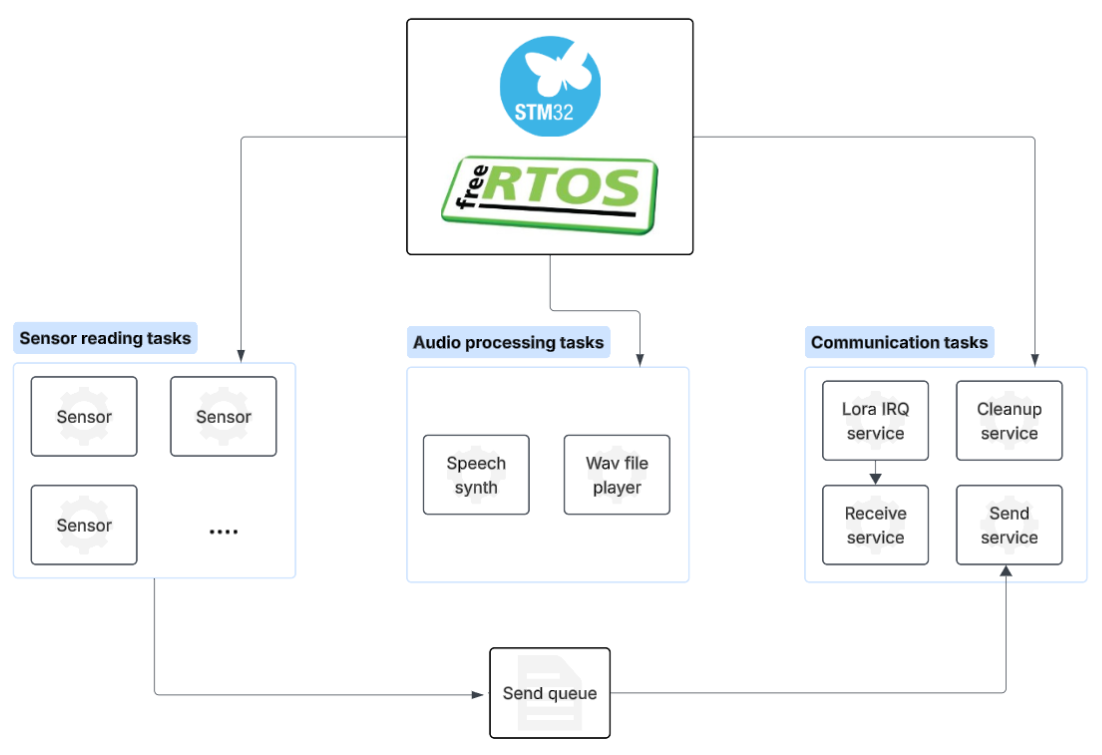
\includegraphics[width=0.45\textwidth]{images/firmware-system-design.png}
\caption{Overview of the FreeRTOS-based firmware architecture}\label{fig:firmware-system}
\end{figure}

\subsection{Overall Architecture}

Figure~\ref{fig:firmware-system} shows three primary functional domains, each implemented as one or more FreeRTOS tasks communicating via inter-task communication mechanisms provided by FreeRTOS.

\subsection{LoRa Communication}
\begin{itemize}
  \item \textbf{IRQ Handler}
    Waits on the SX1276~\cite{sx1276} interrupt line to detect packet RX/TX completion, then gives a binary semaphore.
  \item \textbf{Receive Task}
    Blocks on that semaphore, retrieves incoming packets, decrypts them with hardware-accelerated AES-128 in CTR mode, and forwards them for processing.  
  \item \textbf{Transmit Task}
    Pulls outgoing messages from a FreeRTOS queue, encrypts and formats them, then issues the LoRa send command.
  \item \textbf{Cleanup Task}
    Periodically scans stored packet buffers for timeouts and frees associated heap memory.
\end{itemize}

\subsection{Sensor Management}
Each sensor (e.g.\ temperature, pressure, speed) runs its own task at a low priority. Tasks periodically sample the hardware interface, package reacdings, and enqueues them for transmission.

\subsection{Audio Processign}
\begin{itemize}
  \item \textbf{Speech Synthesis Task}
    A port of \texttt{espeak-ng}~\cite{espeakng} with all file I/O replaced bu in-memory C arrays. Wich dequeues strings from a FreeRTOS queue, synthesises, streams audio to I2S hardware.
  \item \textbf{WAV playback Task}
    Streams hard-coded WAV data (e.g.\ racing flags, standard phrases) to the I2S hardware.
\end{itemize}

\subsection{Power and Memory Management}

All tasks are assigned carefully chosen priorities (Table~\ref{tab:priorities}) so that time-critical communication tasks preempt lower-priority work. We enable FreeRTOS tickless idle to allow the STM32U5 to enter deep sleep whenever the system is idle.

\begin{table}[H]
  \centering
  \caption{Task priorities and stack usage}
  \label{tab:priorities}
  \begin{tabular}{lrr}
    \hline
    Task                     & Priority & Stack (bytes) \\
    \hline
    LoRa IRQ Handler         & 8        & 128            \\
    Speech Synthesis         & 7        & 48\,000        \\
    WAV Playback             & 7        & 256            \\
    LoRa Transmit            & 5        & 128            \\
    Cleanup                  & 5        & 128            \\
    Sensor (each)            & 3        & 256            \\
    \hline
  \end{tabular}
\end{table}

\section{Software Design and Implementation}

This design outlines the software developed for a Raspberry Pi, consisting of two main components: a C++ backend responsible for managing LoRa communication, and a Flutter frontend that delivers a user-friendly interface for message handling and display.

\begin{figure}[H]
\centering
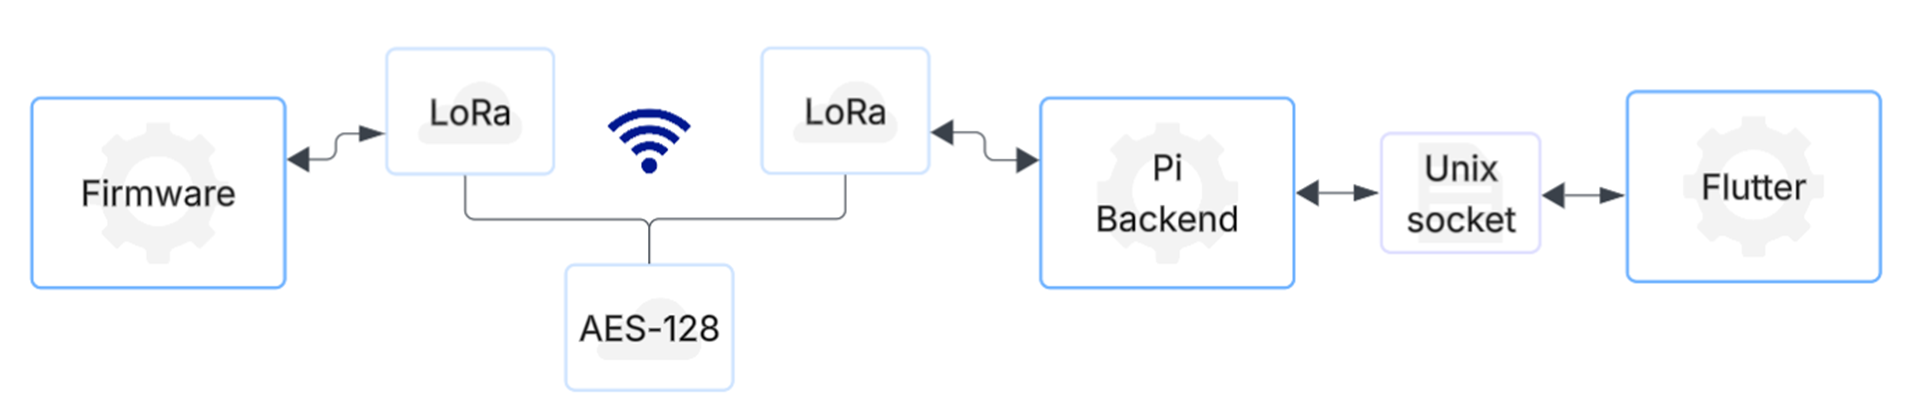
\includegraphics[width=0.45\textwidth]{images/lora-shield.png}
\caption{Overview of the software design}\label{fig:lora-shield}
\end{figure}

\subsection{Backend Implementation}

The backend is implemented in C++ and is responsible for managing the core functionality of the LoRa communication system with the firmware. 
This script is currently designed to run on a Raspberry Pi (RPI), where a shield called the LoRa-GPS HAT~\cite{LoRa-GPS-HAT} is mounted. 
This shield includes a GPS module (not utilized in this project) and an RFM96 LoRa chip~\cite{LoRa module}, a low-power, 
long-range transceiver that operates in the 868\,MHz frequency band.

\subsection{LoRa Communication Layer}

The LoRa communication layer ensures that the backend can send and receive messages over the LoRa network.
Before communication can be established, the interface with the LoRa chip on the shield must be properly configured.

\textbf{SPI Initialization:}

\begin{enumerate}
  \item SPI must be enabled on the Raspberry Pi using the \texttt{raspi-config} utility.
  \item Once enabled, SPI is initialized in the code. The WiringPi library~\cite{WiringPi} is used to access the GPIO pins—specifically, 
  Pin~7 is configured as the interrupt (IRQ) pin for the LoRa chip. After the hardware connection is established, register-level communication is handled through implemented methods such as \texttt{read\_register} and \texttt{write\_register}. Additionally, the \texttt{write\_fifo} method is used to transfer data into the FIFO buffer of the LoRa transceiver.
\end{enumerate}

\textbf{Message Handling:} \\
To support message exchange with the firmware, 
we adapted the same communication library used by the firmware and tailored it to fit the backend's architecture. 
A consistent packet structure is required for interoperability. Each packet includes the following fields: 
\texttt{type}, \texttt{message\_id}, \texttt{fragment\_id}, \texttt{total\_fragments}, \texttt{length}, \texttt{data}, and \texttt{checksum}. 
This structure ensures reliable fragmentation, transmission, and validation of messages between the backend and firmware.
Then to make this more secure we used AES-128 encryption ~\cite{tiny-AES} in CTR mode to encrypt the data field of the packet. 

\subsection{Communication between the Backend and the Frontend}

To establish a smooth and efficient flow of communication between the backend and the frontend, a non-blocking Unix domain socket is used.
This approach enables asynchronous communication, allowing the system to perform multiple operations concurrently without blocking the main 
thread—an essential feature for real-time LoRa communication.

A corresponding socket is also implemented in the Flutter application, enabling the frontend to interact with the backend seamlessly 
and without interrupting its main execution thread.

\textbf{Receiving LoRa Packets from the Firmware:} \\
When a LoRa packet is received from the firmware, the backend handles it using the following sequence:

\begin{enumerate}
  \item An interrupt is immediately triggered by the LoRa module.
  \item The backend processes the received packet.
  \item The processed packet is forwarded to the frontend through the non-blocking Unix domain socket.
  \item The system remains responsive and ready to handle the next incoming LoRa packet.
\end{enumerate}

\subsection{Frontend implementation}

Below is an image showcasing the user interface. The frontend is implemented using Flutter~\cite{flutter}, which enables the development of a responsive and user-friendly UI.

\begin{figure}[H]
\centering
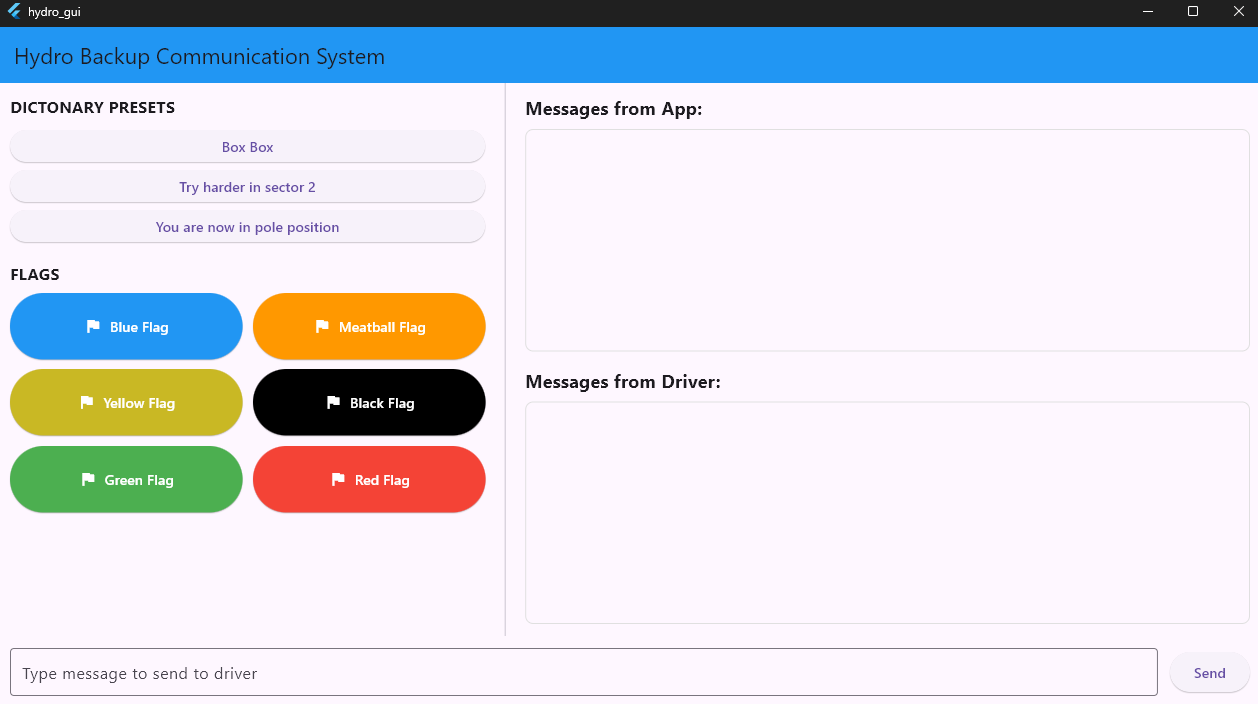
\includegraphics[width=0.45\textwidth]{images/frontend-design.png}
\caption{User interface}\label{fig:frontend-design}
\end{figure}

The interface is composed of several key elements:

\begin{itemize}
    \item Split-view layout with preset messages and flags on the left
    \item Dual message displays showing both sent/app and received messages
    \item An input field for composing custom messages
\end{itemize}

The preset messages and flags are designed for quick access, allowing the user to send predefined commands to the driver efficiently. 
Each flag is associated with a specific ID (e.g., the blue flag corresponds to \texttt{FLAG:1}). 
When the user taps a flag, the corresponding ID is sent to the backend, which forwards it to the firmware. 
The firmware then plays the appropriate \texttt{.wav} file stored on the Nucleo board.

For custom messages, the entered text is transmitted as raw data. 
The firmware receives this message and uses speech synthesis to convert the text into audio output.

On the right side of the interface, received messages from the backend are displayed. 
These may include system notifications, such as error reports or status pings to verify that the driver can receive and acknowledge incoming messages.

\section{Hardware Design and Implementation}

\subsection{System overview}
%De functies van de hardware bestaan uit 6 delen; deze zijn onder andere: voeding, microcontroller, geluid opnemen, geluid produceren, draadloze communicatie, voeding schakelen.
%Dit is buiten de microcontroller voorzien op een PCB in de vorm van een schild passend op een STM32 Nulceo bord met microcontroller.
%Deze onderdelen moeten low power zijn en werken vanuit een 12V voeding.
%De voeding zal bestaan uit een geschakelde voeding die een 3.3V en een 5V zal produceren voor de verdere logica. 
%de microcontroller kan geluid verwerken via een externe ADC (analog digital converter) en geluid uitsturen via een externe DAC (digital analog converter).
%Deze voeding van deze geluids onderdelen kunnen geschakeled worden door de microcontroller door middel van mosfets.
%Dit zorgt ervoor dat als de onderdelen niet gebruikt worden er geen energie verbruikt wordt.
%Via een LoRa module kan de verwerkte spraak verstuurd worden of antvangen worden en afgespeeld.

The hardware functionalities can be divided into six main components: power supply, microcontroller, audio recording, audio playback, wireless communication, and power switching.
Apart from the microcontroller, these components are implemented on a custom PCB designed as a shield compatible with an STM32 Nucleo board.
All components are designed to be low-power and operate from a 12V power source.
The power supply includes a switching regulator that generates both 3.3V and 5V rails to power the remaining circuitry.
Audio input is handled via an external analog-to-digital converter (ADC), while audio output is managed through an external digital-to-analog converter (DAC).
The power to these audio components can be switched on or off by the microcontroller using MOSFETs, allowing the system to conserve energy when the components are not in use.
Processed speech data can be transmitted or received via a LoRa module, and subsequently played back if needed.

\subsection{Power supply}

%De voeding bestaat uit 2 buck converters die de 12V voeding verlagen naar 5V en 3.3V. 
%Hiervoor is gebruik gemaakt van de TPS629203. 
%Deze converter heeft een spanningsbereik tot 17V en levert een maximale stroom van 300mA.
%Door de hoge schakelfrequentie van  kan een hoog rendement bekomen worden. 
%De schakelfrequenite en schakelmodus worden dynamisch bepaald op basis van de belasting.
%Het schakelen kan gebeuren via PWM (puls width modulation) of PFM (pulse frewuency modulation).
%Deze modus noemt AEE (Automatic Efficiency  Enhancement) en zorgt onder andere voor een hoge
% efficientie bij hele kleine duty cycles wat handig is bij een laag stroomverbruik.

The power supply uses two buck converters to step down the 12V input to 5V and 3.3V, based on the TPS629203.
 This converter supports input voltages up to 17V and delivers up to 300mA of output current [5].
 Thanks to its high switching frequency, it achieves excellent efficiency, which is further optimized by dynamically adjusting both the switching frequency and mode depending on the load. It operates in either PWM (Pulse Width Modulation) or PFM (Pulse Frequency Modulation), depending on the current demand. This feature, known as Automatic Efficiency Enhancement (AEE), maintains high efficiency even at very low duty cycles, making it particularly suitable for low-power applications.\\

\subsection{Microcontroller}

%Als microcontroller werd gebruik gemaakt van de STM32U5.
% Deze meest recente generatie van STM32 ultra low power microcontrollers
% is ideaal voor applicaties waar een minimaal stroomverbruik is vereist.
%Ondanks het ultra lage stroomverbruik zijn er uitvoeringen met 4Mb flash memory en 3 Mb SRAM.
%Via meerdere low-power modes kan de microcontroller tijdens het wachten op boodschappen
% en versturen van boodschappen in naar een low power mode gaan waar bepaalde functionaliteiten uitgeschakeld zijn.
%Om te ontwekken uit deze modi wordt een LPGPIO(low-power general-purpose input/output) gebruikt. 
%In deze opstelling is dit een gekoppeld aan een pin van de LoRa module en een digitale input.
%Op deze manier wordt de microcontroller ontwerkt bij het binnenkomen van LoRa data en een
% druk op de talk knop verbonden met de digitale input.

The STM32U5 microcontroller was selected for this design. This latest generation of STM32 ultra-low-power microcontrollers is well-suited for applications that require minimal energy consumption.
Despite its low power profile, certain variants offer up to 4 MB of Flash memory and 3 MB of SRAM, enabling complex processing and data storage [1].
The microcontroller supports multiple low-power modes, allowing it to significantly reduce power consumption during periods of inactivity, such as while waiting to send or receive messages.
Wake-up from these modes is achieved using Low-Power General-Purpose Input/Output (LPGPIO) pins.
In this setup, an LPGPIO pin is connected to both the LoRa module and a digital input. This configuration enables the microcontroller to wake up upon receiving incoming LoRa data or when the talk butto connected to the digital input is pressed.

\subsection{LoRa}

%Voor de draadloze communicatie is gekozen voor LoRa deze technologie is de fysieke laag voor het bekendere LoRaWAN.
%Deze module is gemakkelijk verkrijgbaar en numerous examples and libraries are available online.
%Om deze technology te gebruiken is gekozen voor de RFM96W van Hoperf [6]. Deze compacte PCB is handmatig te solderen en 
%omvat buiten de antenna alle hardware nodig voor LoRa communicatie.
% Communicatie met deze module is mogelijk via SPI en 5 I/O (input/output) pinnen.
%De data die verstuurd moet worden komt via de SPI bus binnen op de module. 
%Indien data ontvangen wordt zal via een I/O pin gemeld worden op binnenkomende data.
%De antenne wordt via een SMA connector verbonden met de PCB. 
%Hierbij is het mogelijk om een antenne met $\frac{\lambda}{2}$ of $\frac{\lambda}{4}$ te gebruiken.
%Indien een antenne voor $\frac{\lambda}{2}$ gebruikt wordt kan deze via een kabel op een andere plaats gebruikt worden.

For wireless communication, LoRa was selected. This technology serves as the physical layer for the more well-known LoRaWAN protocol.
The chosen module, the RFM96W by HopeRF [6], is readily available and supported by numerous examples and open-source libraries online, making integration and development straightforward.
This compact PCB can be hand-soldered and includes all the necessary hardware for LoRa communication, except for the antenna.
Communication with the module is established via the SPI bus and GPIO pins.
Data to be transmitted is sent to the module via the SPI interface, while incoming data is signaled through a dedicated I/O pin.
The antenna is connected to the PCB using an SMA connector. Both $\frac{\lambda}{2}$ and $\frac{\lambda}{4}$ antennas can be used.
A $\frac{\lambda}{2}$ antenna may also be placed remotely using a coaxial cable, allowing for more flexible antenna positioning.

\subsection{ADC}

Om audio in te lezen is gebruik gemaakt van een externe ADC, de PCM1808.


\subsection{DAC}

\subsection{Power switching}

\subsection{PCB}





\section{Testing}

\subsection{Test Setup}
The system was evaluated primarily in a laboratory environment. Key aspects such as power consumption, LoRa communication integrity, and audio output functionality were tested. Most tests were conducted manually, involving the transmission of periodic test messages and monitoring system responses via serial output and audio feedback. Power draw was observed using an inline current measurement tool, and LoRa transmissions were validated using logic analyzers and debug logs.

\subsection{Communication Testing}
To verify LoRa communication, encrypted packets were periodically transmitted and received between two system nodes. Tests confirmed successful decryption, CRC validation, and end-to-end data integrity.

\subsection{Audio Output Testing}
WAV file playback was validated by connecting the system's analog output to external speakers and assessing the clarity of preloaded audio samples. Speech synthesis was tested by transmitting predefined sentences to the device and evaluating intelligibility through blind listening tests. Testers rated intelligibility qualitatively. While overall clarity was sufficient for basic commands, future improvements may include tuning output filters and optimizing speech synthesis parameters for better naturalness.

\section{Conclusion}

\section*{Acknowledgment}
The authors would like to thank the supervising professors for their guidance throughout the development of this project. Special thanks go to the Hydro Team KU Leuven for providing valuable context and support related to the vehicle's communication needs. 

Additionally, the authors used generative AI tools to assist with language refinement and grammar correction during the preparation of this paper.

\begin{thebibliography}{1}
\bibitem{stm32u5}
STMicroelectronics,
\textit{STM32U5-series overview},
2023.
Available: \url{https://www.st.com/en/microcontrollers-microprocessors/stm32u5-series.html}

\bibitem{freertos}
Real Time Engineers Ltd.,
\textit{FreeRTOS Kernel Reference Manual},
2024.
Available: \url{https://www.freertos.org/Documentation/RTOS_book.html}

\bibitem{sx1276}
Semtech Corporation,
\textit{SX1276 LoRa Transceiver IC},
2025.
Available: \url{https://www.semtech.com/products/wireless-rf/lora-connect/sx1276}
\end{thebibliography}


\end{document}
